%!TEX TS-program = xelatex
\documentclass[10pt,oneside]{article}
\usepackage[fontsize=9pt]{scrextend}

\usepackage[english]{babel}

\usepackage{amsmath,amssymb,amsfonts}
\usepackage[utf8]{inputenc}
\usepackage[T1]{fontenc}
\usepackage{stix2}
\usepackage[scaled]{helvet}
\usepackage[scaled]{inconsolata}

\usepackage{lastpage}

\usepackage{setspace}

\usepackage{ccicons}

\usepackage[hang,flushmargin]{footmisc}

\usepackage{geometry}

\setlength{\parindent}{0pt}
\setlength{\parskip}{6pt plus 2pt minus 1pt}

\usepackage{fancyhdr}
\renewcommand{\headrulewidth}{0pt}\providecommand{\tightlist}{%
  \setlength{\itemsep}{0pt}\setlength{\parskip}{0pt}}

\makeatletter
\newcounter{tableno}
\newenvironment{tablenos:no-prefix-table-caption}{
  \caption@ifcompatibility{}{
    \let\oldthetable\thetable
    \let\oldtheHtable\theHtable
    \renewcommand{\thetable}{tableno:\thetableno}
    \renewcommand{\theHtable}{tableno:\thetableno}
    \stepcounter{tableno}
    \captionsetup{labelformat=empty}
  }
}{
  \caption@ifcompatibility{}{
    \captionsetup{labelformat=default}
    \let\thetable\oldthetable
    \let\theHtable\oldtheHtable
    \addtocounter{table}{-1}
  }
}
\makeatother

\usepackage{array}
\newcommand{\PreserveBackslash}[1]{\let\temp=\\#1\let\\=\temp}
\let\PBS=\PreserveBackslash

\usepackage[breaklinks=true]{hyperref}
\hypersetup{colorlinks,%
citecolor=blue,%
filecolor=blue,%
linkcolor=blue,%
urlcolor=blue}
\usepackage{url}

\usepackage{caption}
\setcounter{secnumdepth}{0}
\usepackage{cleveref}

\usepackage{graphicx}
\makeatletter
\def\maxwidth{\ifdim\Gin@nat@width>\linewidth\linewidth
\else\Gin@nat@width\fi}
\makeatother
\let\Oldincludegraphics\includegraphics
\renewcommand{\includegraphics}[1]{\Oldincludegraphics[width=\maxwidth]{#1}}

\usepackage{longtable}
\usepackage{booktabs}

\usepackage{color}
\usepackage{fancyvrb}
\newcommand{\VerbBar}{|}
\newcommand{\VERB}{\Verb[commandchars=\\\{\}]}
\DefineVerbatimEnvironment{Highlighting}{Verbatim}{commandchars=\\\{\}}
% Add ',fontsize=\small' for more characters per line
\usepackage{framed}
\definecolor{shadecolor}{RGB}{248,248,248}
\newenvironment{Shaded}{\begin{snugshade}}{\end{snugshade}}
\newcommand{\KeywordTok}[1]{\textcolor[rgb]{0.13,0.29,0.53}{\textbf{#1}}}
\newcommand{\DataTypeTok}[1]{\textcolor[rgb]{0.13,0.29,0.53}{#1}}
\newcommand{\DecValTok}[1]{\textcolor[rgb]{0.00,0.00,0.81}{#1}}
\newcommand{\BaseNTok}[1]{\textcolor[rgb]{0.00,0.00,0.81}{#1}}
\newcommand{\FloatTok}[1]{\textcolor[rgb]{0.00,0.00,0.81}{#1}}
\newcommand{\ConstantTok}[1]{\textcolor[rgb]{0.00,0.00,0.00}{#1}}
\newcommand{\CharTok}[1]{\textcolor[rgb]{0.31,0.60,0.02}{#1}}
\newcommand{\SpecialCharTok}[1]{\textcolor[rgb]{0.00,0.00,0.00}{#1}}
\newcommand{\StringTok}[1]{\textcolor[rgb]{0.31,0.60,0.02}{#1}}
\newcommand{\VerbatimStringTok}[1]{\textcolor[rgb]{0.31,0.60,0.02}{#1}}
\newcommand{\SpecialStringTok}[1]{\textcolor[rgb]{0.31,0.60,0.02}{#1}}
\newcommand{\ImportTok}[1]{#1}
\newcommand{\CommentTok}[1]{\textcolor[rgb]{0.56,0.35,0.01}{\textit{#1}}}
\newcommand{\DocumentationTok}[1]{\textcolor[rgb]{0.56,0.35,0.01}{\textbf{\textit{#1}}}}
\newcommand{\AnnotationTok}[1]{\textcolor[rgb]{0.56,0.35,0.01}{\textbf{\textit{#1}}}}
\newcommand{\CommentVarTok}[1]{\textcolor[rgb]{0.56,0.35,0.01}{\textbf{\textit{#1}}}}
\newcommand{\OtherTok}[1]{\textcolor[rgb]{0.56,0.35,0.01}{#1}}
\newcommand{\FunctionTok}[1]{\textcolor[rgb]{0.00,0.00,0.00}{#1}}
\newcommand{\VariableTok}[1]{\textcolor[rgb]{0.00,0.00,0.00}{#1}}
\newcommand{\ControlFlowTok}[1]{\textcolor[rgb]{0.13,0.29,0.53}{\textbf{#1}}}
\newcommand{\OperatorTok}[1]{\textcolor[rgb]{0.81,0.36,0.00}{\textbf{#1}}}
\newcommand{\BuiltInTok}[1]{#1}
\newcommand{\ExtensionTok}[1]{#1}
\newcommand{\PreprocessorTok}[1]{\textcolor[rgb]{0.56,0.35,0.01}{\textit{#1}}}
\newcommand{\AttributeTok}[1]{\textcolor[rgb]{0.77,0.63,0.00}{#1}}
\newcommand{\RegionMarkerTok}[1]{#1}
\newcommand{\InformationTok}[1]{\textcolor[rgb]{0.56,0.35,0.01}{\textbf{\textit{#1}}}}
\newcommand{\WarningTok}[1]{\textcolor[rgb]{0.56,0.35,0.01}{\textbf{\textit{#1}}}}
\newcommand{\AlertTok}[1]{\textcolor[rgb]{0.94,0.16,0.16}{#1}}
\newcommand{\ErrorTok}[1]{\textcolor[rgb]{0.64,0.00,0.00}{\textbf{#1}}}
\newcommand{\NormalTok}[1]{#1}

\newlength{\cslhangindent}
\setlength{\cslhangindent}{1.5em}
\newlength{\csllabelwidth}
\setlength{\csllabelwidth}{3em}
\newenvironment{CSLReferences}[3] % #1 hanging-ident, #2 entry spacing
 {% don't indent paragraphs
  \setlength{\parindent}{0pt}
  % turn on hanging indent if param 1 is 1
  \ifodd #1 \everypar{\setlength{\hangindent}{\cslhangindent}}\ignorespaces\fi
  % set entry spacing
  \ifnum #2 > 0
  \setlength{\parskip}{#2\baselineskip}
  \fi
 }%
 {}
\usepackage{calc} % for \widthof, \maxof
\newcommand{\CSLBlock}[1]{#1\hfill\break}
\newcommand{\CSLLeftMargin}[1]{\parbox[t]{\maxof{\widthof{#1}}{\csllabelwidth}}{#1}}
\newcommand{\CSLRightInline}[1]{\parbox[t]{\linewidth}{#1}}
\newcommand{\CSLIndent}[1]{\hspace{\cslhangindent}#1}\usepackage[table,dvipsnames]{xcolor}

\geometry{includemp,
            letterpaper,
            top=2.4cm,
            bottom=2.4cm,
            left=1.0cm,
            right=1.0cm,
            marginparwidth=5cm,
            marginparsep=1.0cm}

\usepackage[singlelinecheck=off]{caption}

\captionsetup{
  font={small},
  labelfont={bf},
  format=plain,
  labelsep=quad
}

\usepackage{floatrow}

\floatsetup[figure]{margins=hangright,
              facing=no,
              capposition=beside,
              capbesideposition={center,outside},
              floatwidth=\textwidth}

% \floatsetup[table]{margins=hangright,
%              facing=no,
%              capposition=beside,
%              capbesideposition={center,outside},
%              floatwidth=\textwidth}

\pagestyle{plain}

\setcounter{secnumdepth}{5}

\usepackage{titlesec}

\titleformat{\section}[block]
{\normalfont\large\sffamily}
{\thesection}{.5em}{\titlerule\\[.8ex]\bfseries}

\titleformat{\subsection}[runin]
{\normalfont\fontseries{b}\selectfont\filright\sffamily}
{\thesubsection.}{.5em}{}

\titleformat{\subsubsection}[runin]
{\normalfont\itshape\rmfamily\bfseries}{\thesubsubsection}{1em}{}

\fancypagestyle{firstpage}
{
   \fancyhf{}
   \renewcommand{\headrulewidth}{0pt}
   \fancyfoot[R]{\footnotesize\ccby}
   \fancyfoot[L]{\footnotesize\sffamily\today}
}

\fancypagestyle{normal}
{
  \fancyhf{}
  \fancyfoot[R]{\footnotesize\sffamily\thepage\ of \pageref*{LastPage}}
}

\usepackage{tikz}
\begin{document}
\tikz [remember picture, overlay] %
\node [shift={(-0.6in,1.1cm)},scale=0.2,opacity=0.4] at (current page.south east)[anchor=south east]{
\includegraphics{logo}};%
\pagestyle{normal}
\thispagestyle{firstpage}

\newcommand{\colorRule}[3][black]{\textcolor[HTML]{#1}{\rule{#2}{#3}}}

\noindent {\LARGE \textbf{\textsf{Template to prepare preprints and
manuscripts using markdown and github actions}}}

\medskip
\begin{flushleft}
{\small
%
\href{https://orcid.org/0000-0002-6506-6487}{Michael D.\,Catchen}%
%
\,\textsuperscript{1,2}, %
\href{https://orcid.org/0000-0002-6004-4027}{Laura\,Pollock}%
%
\,\textsuperscript{1,2}, %
\href{https://orcid.org/0000-0002-0735-5184}{Timothée\,Poisot}%
%
\,\textsuperscript{3,2}, %
\href{https://orcid.org/0000-0001-6075-8081}{Andrew\,Gonzalez}%
%
\,\textsuperscript{1,2}
\vskip 1em
\textsuperscript{1}\,McGill University; \textsuperscript{2}\,Québec
Centre for Biodiversity Sciences; \textsuperscript{3}\,Université de
Montréal\\
\vskip 1em
\textbf{Correspondance to:}\\
Michael D. Catchen --- \texttt{michael.catchen@mcgill.ca}\\
}
\end{flushleft}

\vskip 2em
\makebox[0pt][l]{\colorRule[CCCCCC]{2.0\textwidth}{0.5pt}}
\vskip 2em
\noindent

\marginpar{\vskip 1em\flushright
{\small{\bfseries Keywords}:\par
pandoc\\pandoc-crossref\\github actions\\}
}




        {\bfseries Abstract:}\,TBD\\%
    

\vskip 2em
\makebox[0pt][l]{\colorRule[CCCCCC]{2.0\textwidth}{0.5pt}}
\vskip 2em

\hypertarget{introduction}{%
\section{Introduction}\label{introduction}}

Earth's ecosystems are changing due to human activity.

However, we currently lack the data collected in a systematic way to
adaquetly attribute change in biodiversity to particular drivers, and to
filter out inherent temporal variation in ecological processes from
deviations toward non-stationarity (TODO: wording)
(\textbf{AndyDNAPaper?}).

Sampling is expensive.

What is a BON? Talk about other important aspects of this framework. We
want the data to be open. We want to encourage colloboration across
scales. Not top-down.

\hypertarget{methods}{%
\section{Methods}\label{methods}}

\hypertarget{combining-many-geospatial-layers-into-a-priority-map}{%
\subsection{Combining many geospatial layers into a priority
map}\label{combining-many-geospatial-layers-into-a-priority-map}}

A set of geospatial layers, which potentially represent many different
types of information. Here we consider each layer to fall into one of
three categories: (1) ecological layers, which represent information
about biological processes, e.g.~species richness, trend in abundance,
uncertainty in species occurrence, etc. (2) environmental layers, which
represent information about the abiotic environment, e.g.~climatic
information, land-cover, elevation, climate velocity and uniqueness, and
son. Finally, (3) cost layers: e.g.~the physical accessability of
certain locations, the amount of money per unit of time spend sampling a
given location, etc. We denote the value of an arbitrary layer \(L_i\)
at the coordinate \((x,y)\) as \(L_i^{(x,y)}\). We also denoted a
generic function \(g(L_i)\) where returns the group (ecological,
environmental, cost) that the particular \(L_i\) belongs to. We also
define a set of targets, which are the objective information to be
obtained via sampling. (examples here).

The fundemental objects here are the weights matrix \(\mathbf{W}\), and
mixing vectors \(\gamma\) and \(\phi\). The weights matrix
\(\mathbf{W}\) is an \(\mathcal{L} \times \mathcal{T}\) matrix, where
\(\mathcal{L}\) and \(\mathcal{T}\) are the number of layers and targets
respectively. The value of \(\mathbf{w}_{i,t}\) is the relative
importance of the \(i\)-th layer to the \(t\)-th target compared to all
of the other layers in the group the \(i\)-th layer is in, \(g(L_i)\).
From this, and the layer group mixing vector \(\phi\), we can compute
single layers for each target, where we similarly denote the value
\(i\)-th target at location \((x,y)\) as \(T_i^{(x,y)}\). This can be
computed as \[T_i^{(x,y)} = \sum_j \gamma_{g(L_j)}
\cdot \mathbf{w}_{j,i} \cdot L_j^{(x,y)}\]or in slightly more compact
matrix form

\[\vec{\mathbf{T}}^{(x,y)} = \mathbf{W}^T(\vec{\gamma}^* \circ \vec{\mathbf{L}}^{(x,y)})\]

where \(\vec{\gamma}^*\) is a vector of length \(\mathcal{L}\) where
\(\gamma_i^* = g(L_i)\).

Finally, these target layers can then be combined into a single map as a
weighted average based on the target mixing weights \(\phi\), i.e.~the
priorty map \(\mathbf{P}\) at \((x,y)\) can be computed as
\[\mathbf{P}^{(x,y)} = \sum_i \phi_i
T_i^{(x,y)}\] or in its complete matrix form

\[\mathbf{P}^{(x,y)} = \mathbf{W}^T (\vec{\gamma}^* \circ \mathbf{L}^{(x,y)}) \cdot \phi \]

where \(\circ\) is the element-wise product and \(\cdot\) is the inner
product

\begin{figure}
\hypertarget{fig:concept}{%
\centering
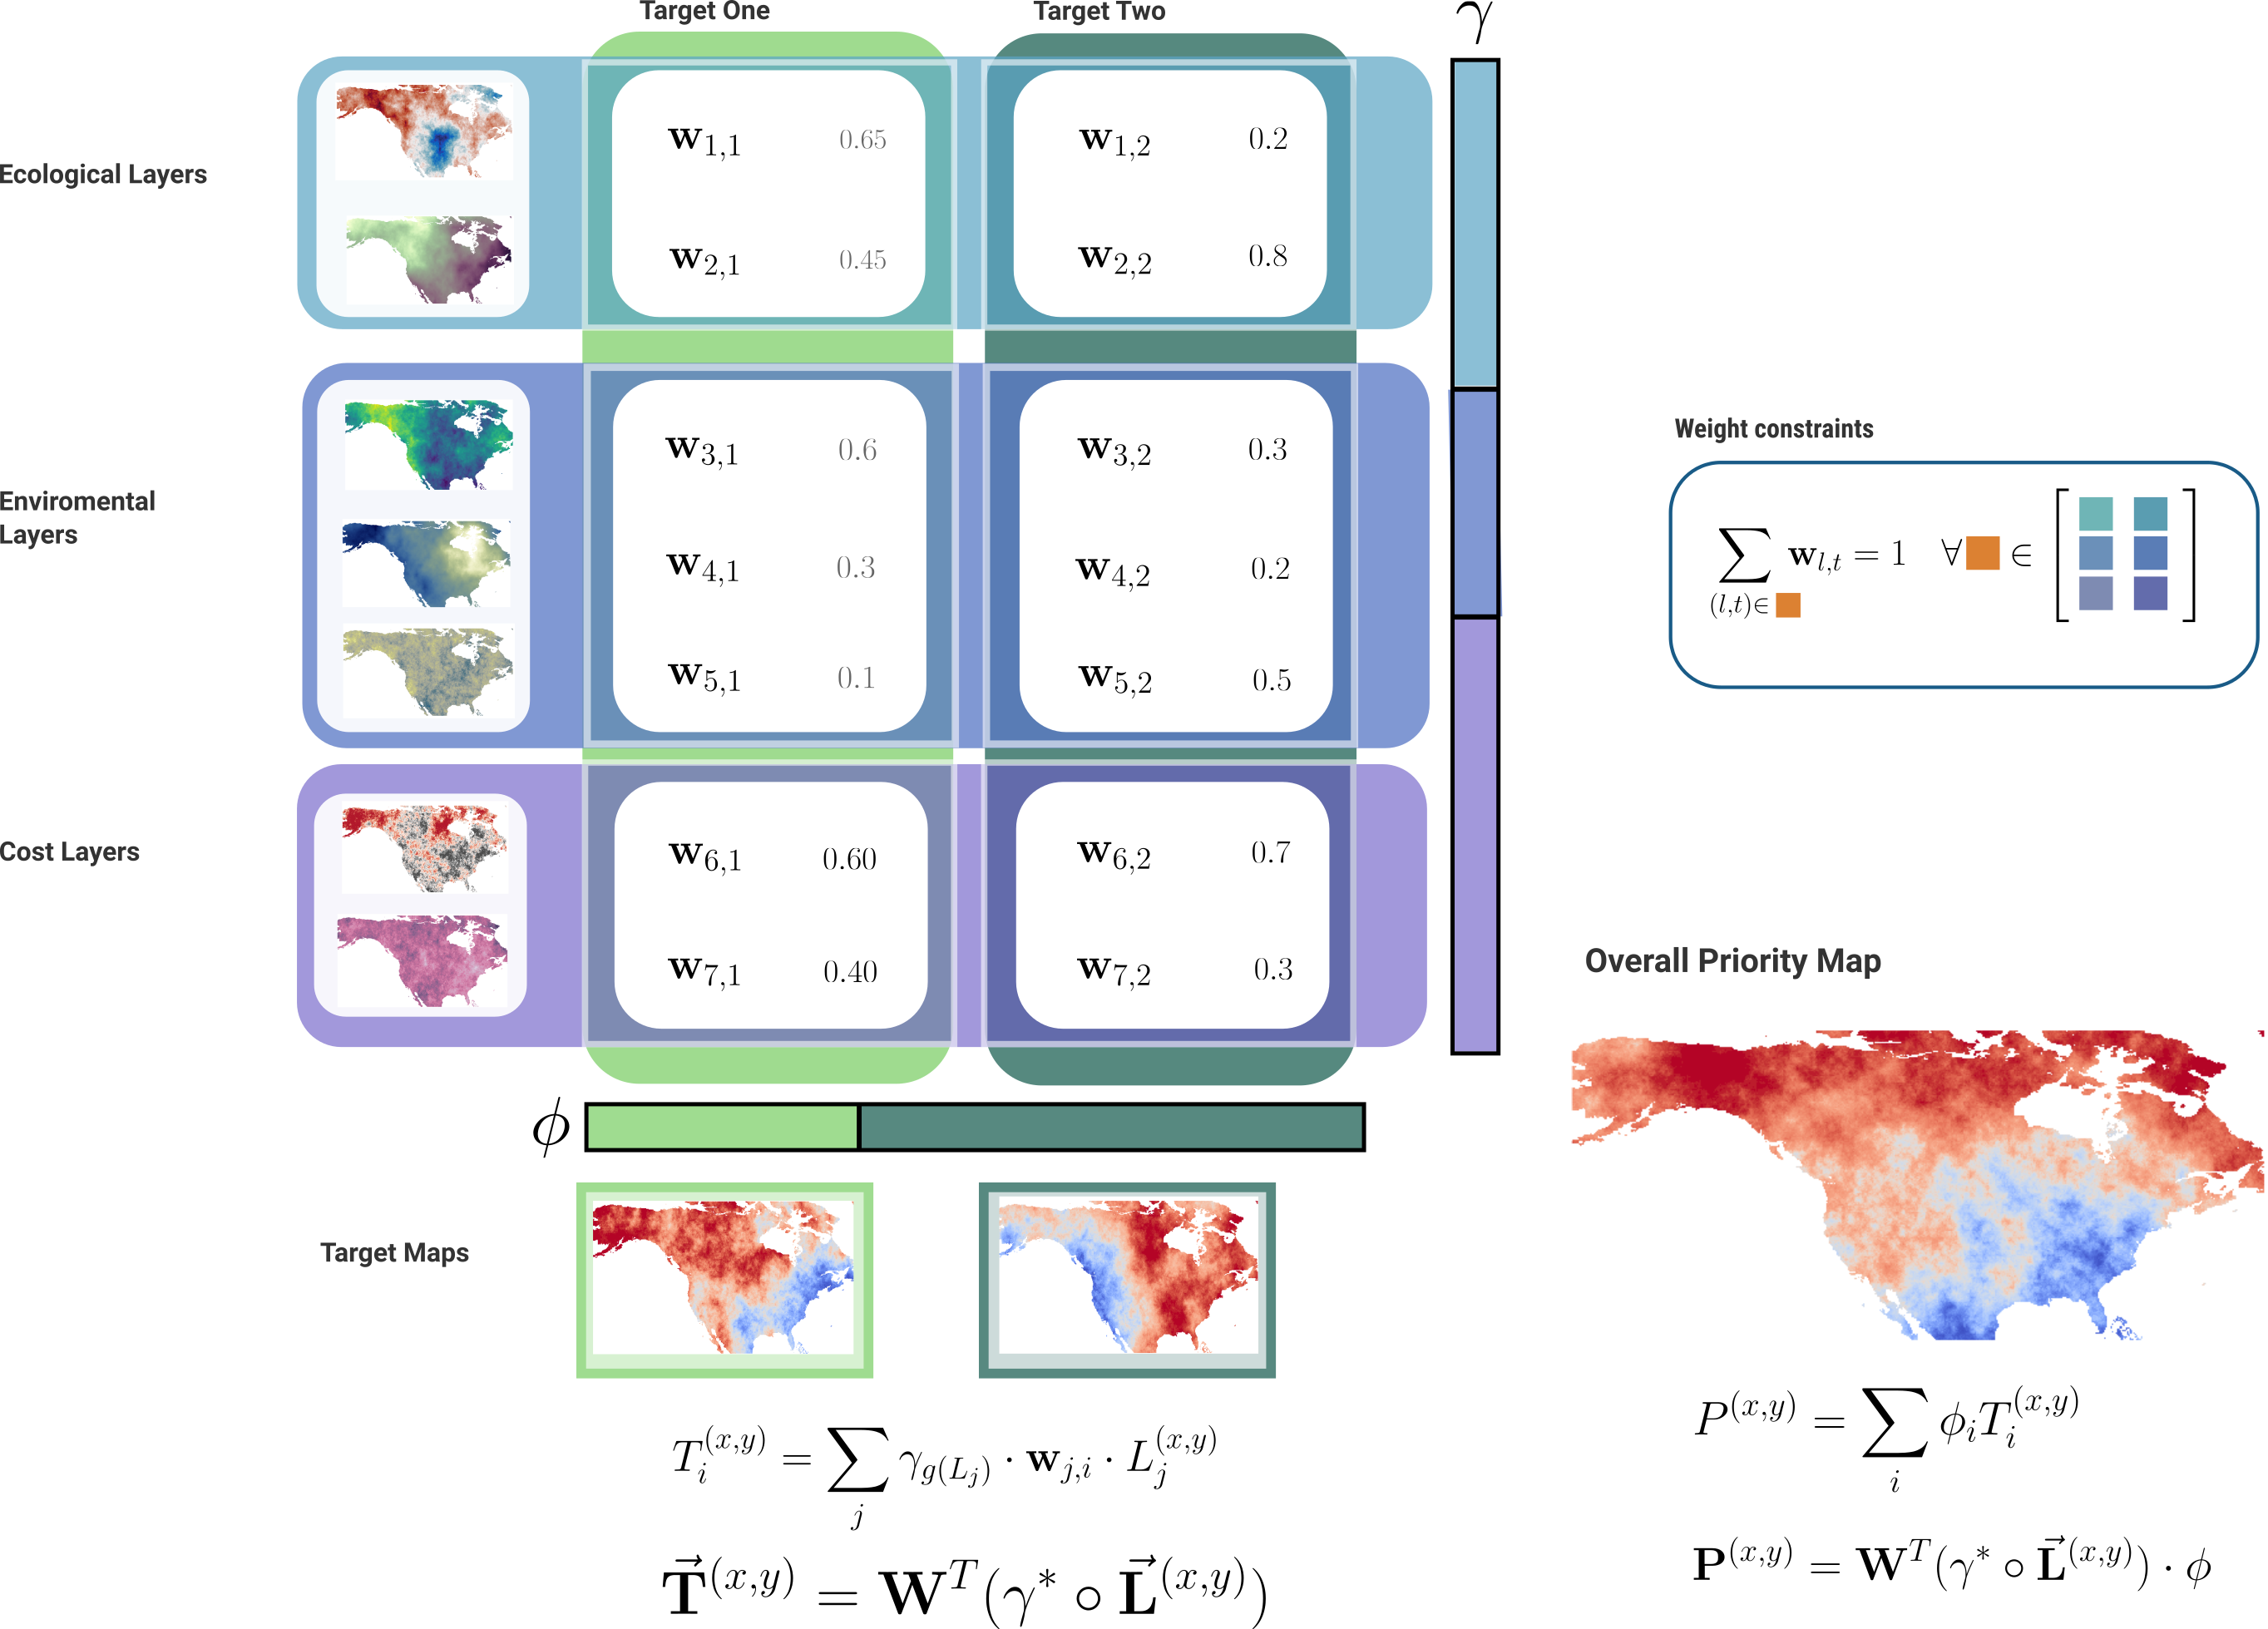
\includegraphics{./figures/weights_concept.png}
\caption{todo}\label{fig:concept}
}
\end{figure}

\hypertarget{point-selection-algorithms}{%
\subsection{Point selection
algorithms}\label{point-selection-algorithms}}

There is a long history of discourse in the literature about choosing a
set of coordinates within a spatial domain that will result in a
``best'' sample.

\begin{itemize}
\tightlist
\item
  Environmental uniqueness
\item
  Spatial balance
\item
  Whatever the fuck cube sampling is doing
\item
  Particular scale-dependence weirdness in ecology
\end{itemize}

\hypertarget{choosing-and-optimizing-weights}{%
\subsection{Choosing and optimizing
weights}\label{choosing-and-optimizing-weights}}

There are a lot of caveats here.

\begin{itemize}
\tightlist
\item
  Rarely is there relevant available data from which to derive an
  evidence-based choice of the relative importance of each layer toward
  sampling targets.
\item
  Often knowledge of species life-history matters for this, requires
  experts on particular species
\item
  There is no a priori reason to believe there will be a positive
  trade-off possible between two targets.
\item
  A particular choice of weight matrix may produce a priority map that
  is very sensitive to minor changes in the weights
\item
  We should try to validate that our sampling sites work well, but this
  is a chicken and egg problem with our current data. So we want a
  max-entropy approach to real distributions from which we sample
  possible realized sampling outcomes and compare as we tweak weights.
\item
  Need to assert the constraint that
  \[\frac{\partial \mathbb{L}_i}{\partial
  T_i}>0\] or otherwise that means the weights are not actually suited
  toward targets
\end{itemize}

\hypertarget{target-tradeoffs}{%
\subsubsection{Target tradeoffs}\label{target-tradeoffs}}

\begin{figure}
\hypertarget{fig:tradeoff}{%
\centering
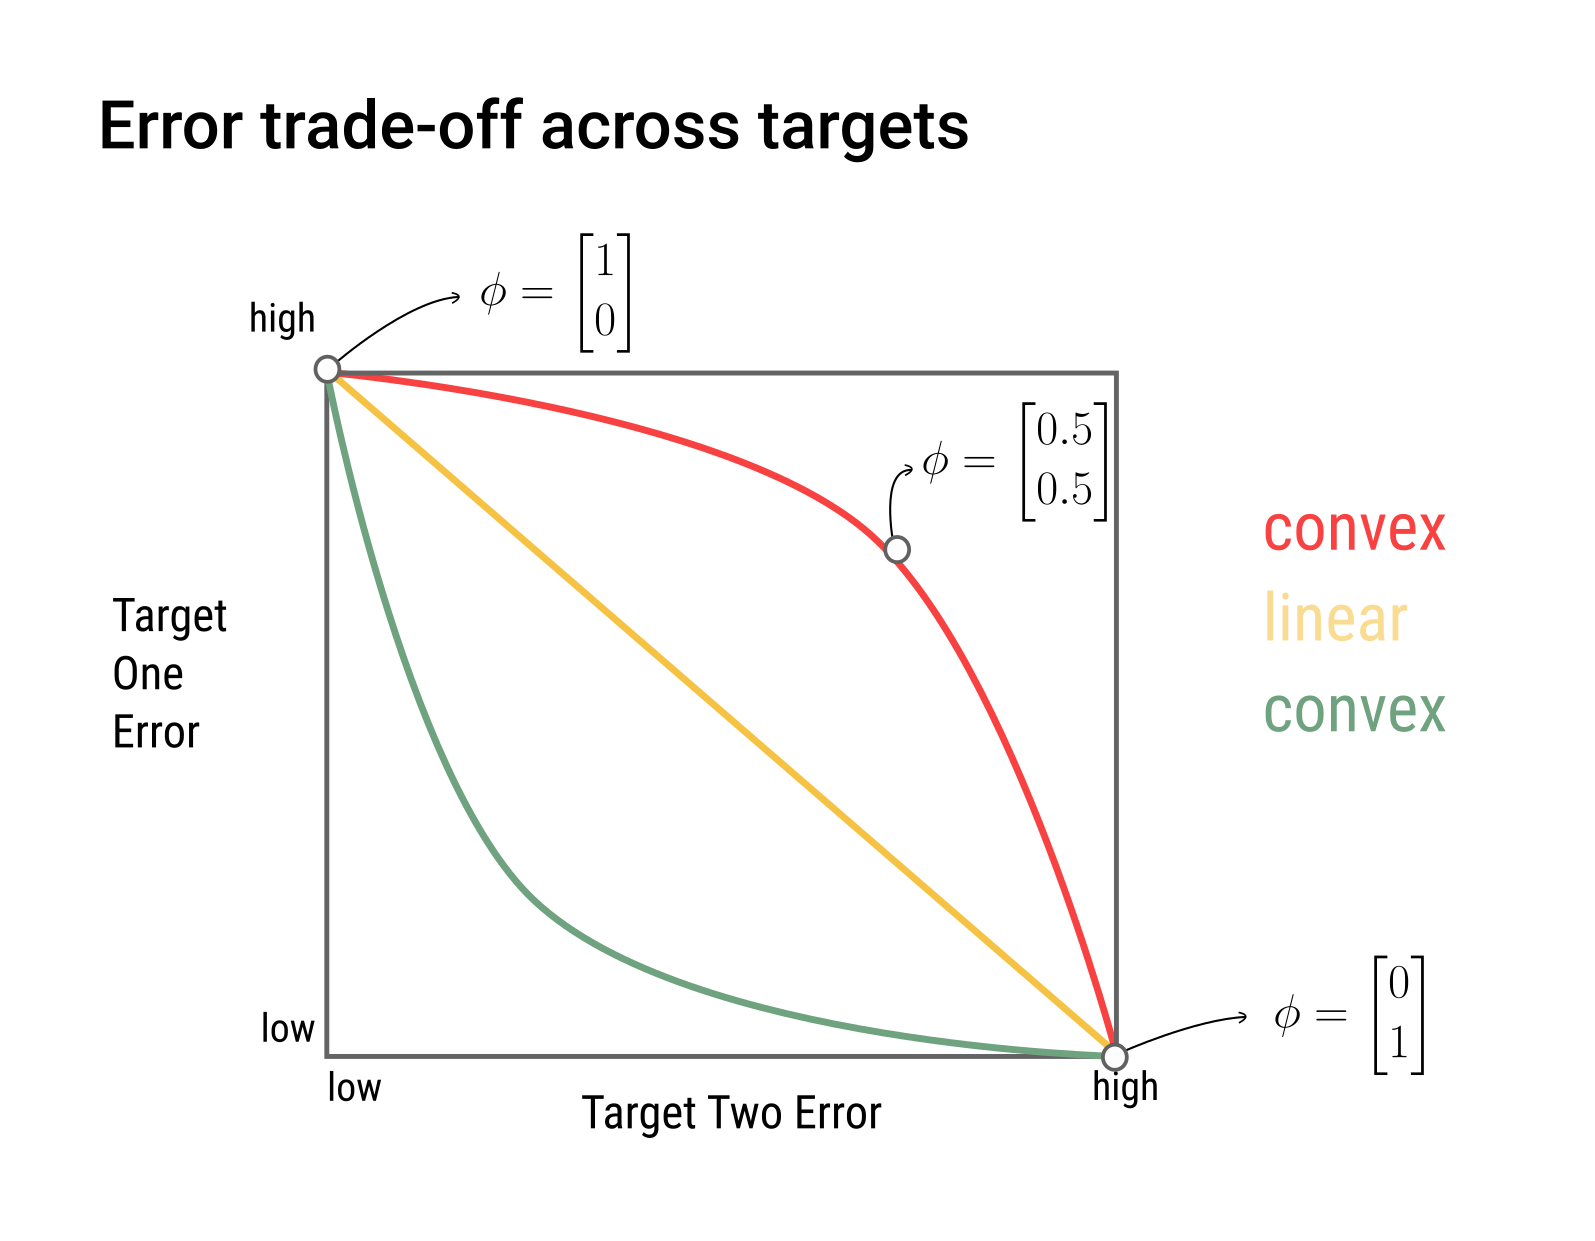
\includegraphics{./figures/tradeoff_concept.png}
\caption{todo}\label{fig:tradeoff}
}
\end{figure}

\hypertarget{sensitivity-analysis}{%
\subsubsection{Sensitivity analysis}\label{sensitivity-analysis}}

\hypertarget{validation-through-simulation-of-the-sampling-process}{%
\subsubsection{Validation through simulation of the sampling
process}\label{validation-through-simulation-of-the-sampling-process}}

\hypertarget{case-study-bird-or-perhaps-non-migratory-species-tbd-in-quebec}{%
\section{Case study: bird (or perhaps non migratory?) species TBD in
Quebec}\label{case-study-bird-or-perhaps-non-migratory-species-tbd-in-quebec}}

\hypertarget{discussion}{%
\section{Discussion}\label{discussion}}

\end{document}
